\newpage

\chapter{Introduction}

The evolution of opinions in multi-agent systems is a well-studied field. In these systems, agents share information in order to reach a consensus. Opinion dynamics focusses on methods for a single agent to combine information from the population to formulate its own beliefs. However, little attention is paid to the content of the information that is broadcast, with agents often revealing the full and exact nature of their beliefs. Such openness is both a lack of privacy and a lack of precision, as an agent might share more information than is relevant. To mitigate this, it is possible to structure the information that is shared; only the most pertinent material that will persuade an agent to change their opinion to align more closely with the new information will be broadcast.

The provision of a structure to the design of communications between agents also improves a current affliction of AI. The rationale behind an agents decision is often unclear~\cite{Doran2017WhatPerspectives}. Hence, it is important to understand the process the agent has undergone to formulate its beliefs, in order to clarify the reason behind its decisions. A structure also improves the understanding of the decision-making process of a population as a whole, such as a swarm of robots that must reach a decision that is best for the group. This paper studies the effects of persuasion on the evolution of opinions in a virtual population. 

Persuasion in human interactions is well studied qualitatively, revealing it to be a multi-faceted phenomenon. One of the most prevalent definitions is as follows:

\begingroup
\addtolength\leftmargini{0.1in}
\begin{quote}
    \textit{Persuasion refers to any change in attitudes that results from exposure to a communication.} \cite{Petty1986CommunicationChange}
\end{quote}
\endgroup


Models are proposed in~\cref{sect:speaker_models} that provide structure to the creation of a communication, and mechanisms for changes in attitude are discussed in~\cref{sect:listener_models}. 

The qualitative features of persuasion are ill-defined quantitatively, making them difficult to incorporate directly into these models. The Elaboration Likelihood Model (ELM) categorises these features into two main ``routes'' for persuasion~\cite{Petty1997ThePsychology}: the Peripheral and the Central Route. The Peripheral Route describes influence that is achieved indirectly, through invoking a positive sentiment that an individual might associate with a notion or object. This method aims to alter a person's attitude subconsciously and often results in only temporary changes in attitude. The Central Route is the more direct approach with arguments and reasons being exchanged without pretence. Due to the temporary and vague nature of the persuasion through the Peripheral Route, it is this Central Route that motivates the work that follows. 

In order to model influence via the Central Route, it is important to understand what variables impact it. For instance, the ELM describes a spectrum of the listener's predisposition to apply significant cognitive effort toward analysing an argument. Those who prefer to dissect new information are most responsive to a strong argument, with few flaws, no matter who presents it. Alternatively, those indisposed to effortful thought surrounding an argument are much more likely to respond positively to the argument if it comes from a source they believe to be expert and reliable. Another impactful factor is the mood of the recipient of an argument; those in a good mood are more likely to accept the argument, while those in a more negative frame of mind are more prone to counter-arguing~\cite{Petty1997ThePsychology}. 

The importance of understanding these routes in the context of this report can be demonstrated with an example. Consider a psychologist and their patient. If the patient were to hold a set of destructive and dangerous beliefs, it is the psychologist's duty to persuade the patient to alter their beliefs so as to improve their health. Equivalently, if an artificial agent were to hold a set of destructive and dangerous beliefs, it is the duty of the designer to persuade the agent to alter its beliefs to be closer to those intended.  Therefore, instead of resetting such an agent and destroying its knowledge base, it is plausible that one could persuade the agent to alter its beliefs with a rational argument. 

One of the closest technological approximations to a human mind at present are Deep Neural Networks. Therefore, an analogue to human persuasion can be found there. For instance, several prominent technology companies are pursuing deep learning as a method for complex communication techniques, of which persuasion is a key element~\cite{Dulac-Arnold2015DeepSpaces, Lowe2019OnCommunication, Guo2017LearningTexts}. For instance, researchers have investigated the use of SVM's to quantify the persuasive and rhetorical power of speeches by US presidential candidates. The research established differences in the persuasiveness of Democratic and Republican candidates based only on four-sentence chunks of their speeches~\cite{Strapparava2010PredictingDiscourses}. The following examples of persuasive technology are from Facebook, IBM and Google respectively.

Facebook has explored neural networks capable of persuasion in the form of natural language negotiation. The researchers analyse a number of possible factors in successful negotiations, including persuasion~\cite{Lewis2017DealDialogues}. Here, the authors attempt to train a pair of networks to negotiate a deal. Each network was given an inventory of arbitrary objects and values. Their objective was to trade items with one another in order to obtain a particular item. They were trained using a dataset of transcriptions of crowd-sourced interpersonal deal-making. This project failed to create agents proficient enough in the use of natural language to be successful. Not only this, the agents also learned to deceive their counterparts. They would systematically understate the value of the object they were targeting attempting to persuade their opponent to give them the best possible deal~\cite{Lewis2017DealDialogues}. This was due to the presence of deception in the training data. Similar behaviour can be observed in the field of experimental economics in~\cite{Smith1976ExperimentalTheory}, a seminal paper on market games. Here, the participants were assigned the role of buyer or seller in a continuous double auction and tasked with making a deal. It was found that the buyers would naturally bid lower than their limit price, and the sellers would do the opposite.

The state-of-the-art in persuasive deep learning methods is Project Debater from IBM, which provides a competitive debating engine. Given a topic and a short amount of time, it can generate a compelling narrative in support of the claim it intends to make (see~\cite{Hou2017ArgumentModel, Mass2018WordSpeech} for more detail). The agent's goal is both to persuade the judges and to respond to the opponent in a formal debating style. To achieve this, the agent is trained on a vast corpus of publicly available debates, transcripts and Wikipedia articles. The agent must identify the most salient aspects of a sentence for the claim in question, extract that information, determine its relevance, and then incorporate it into a compelling speech~\cite{Levy2018TowardsSupervision}. The ``convincingness'' of this speech is learned from a dataset of human debates labelled by professional debaters who determine the relative ``convingness'' of one motion against another~\cite{Habernal2016WhichLSTM}. The authors conclude that this is an effective tool in quantifying the power of an argument and that the errors in the results are likely attributed to ambiguous topics rather than significant flaws in the design of the network. This project also incorporates novel aspects of speech recognition into both the agent's ability to comprehend its opponent's assertions and to rebut them. Whereas previous attempts at sentiment analysis were trained using only text-based transcriptions of public debates, Project Debater extends this to auditory data. This captures the tonality of the speaker so as to better comprehend the claim and sentiment of the argument. The results of this work are preliminary but show that the field of listening comprehension can be incorporated into artificial argumentation and reasoning.


Despite their communicative aptitude, neural networks are vulnerable to targeted adversarial attacks on their decision-making processes. A sufficiently trained network can assign a specific label to a given input. It can also be persuaded to assign a different label if there is a particular adversarial perturbation to that same input. For example, consider a neural network trained to recognise a wide variety of images~\cite{Krizhevsky2012ImageNetNetworks}. \Cref{fig:adversarial_patch} shows an example of such a classifier. Upon receiving an image of a banana, it is the estimation of the network that the image shows a banana. However, when the input is altered, the network changes the label it assigns, incorrectly believing that the image now shows a toaster~\cite{Goodfellow2014ExplainingExamples, Brown2017AdversarialPatch}. The scene-independent nature of this attack highlights a weakness in the decision-making ability of some neural networks. Here, the attackers exploit the network's tendency to focus on the most salient parts of an image and then base its classification heavily on those sections. \Cref{fig:adversarial_patch} shows that the output of the classifier is incorrect when the sticker is added as it recognises the sticker as the most relevant part of the input image. This change of label is an example of persuasion in an adversarial setting. It is especially potent as the attack is not dependent on the input, but on the network architecture, shifting the focus of the classifier regardless of the scene it is placed in. 



\begin{figure}[ht]
    \centering
    \includegraphics[trim={0, 7mm, 0, 0}, clip, width=0.7\textwidth]{Images/Misc/AdversarialPatches.png}
    \caption{An example of an adversarial patch applied to fool a deep neural network performing object recognition. The network can be seen correctly classifying the object contained within the first image, but when the patch is introduced. The network instead focuses on the patch, incorrectly believing it to be highly relevant in the classification, and thereby ignoring the actual image intended for classification, in this case, a banana~\cite{Brown2017AdversarialPatch}. }
    \label{fig:adversarial_patch}
\end{figure}


There is an extensive literature in the area of opinion dynamics, as it is a useful tool to employ in the analysis of social networks and swarm robotics. Understanding the evolution of ideas and motivations in a population is essential for creating rational and consistent behaviour in groups. A broad description of rationality dictates that an agent must be autonomous, sociable, proactive and reactive~\cite{Genesereth1994SoftwareAgents, Castelfranchi1995GuaranteesArchitecture}. Under these tenets, the agents adhere to a set of simple rules and work cohesively towards the collective goal of the group. This is accomplished without central oversight producing results more complex than any agent could create alone~\cite{Rawls1971AJustice}. A requirement for this is that the majority of the population agrees on the best procedure to follow~\cite{Baronchelli2018ThePrimer}. A unanimous agreement of this nature is referred to as global consensus while an agreement within a subset of the population is referred to as local consensus.


The work of~\cite{Parker2009CooperativeProblem} gives an example of the above, describing a population of agents acting without a central authority. This creates a robust population; they are sufficiently autonomous so as not to be incapacitated should a central node fail. The agents must reach a global consensus in order to achieve their goals. In this example, the population must agree on the location of a nest site. Inspiration for this was drawn from naturally occurring swarms of ant and bee colonies~\cite{Pratt2005BehavioralCurvispinosus, List2009IndependenceSwarms}. In~\cite{Parker2009CooperativeProblem}, the agents follow a set of rules for sharing and discovering new information. This enables them to influence one another to adopt a new set of attitudes that best suit the needs of the colony. This change in attitude demonstrates the importance of persuasion in this population, as defined by~\cite{Petty1986CommunicationChange}. It suits the colony to collectively pursue one single desired outcome rather than dividing their resources in disparate pursuits of multiple unrelated goals. In short, it is better to work in concert toward a goal than in discord, even if the ultimate goal is potentially sub-optimal. This is only made possible through effective affective communication of opinions between the agents, though it can likely be refined. 

The opinion of a single agent can be mathematised using aspects of uncertainty modelling, facilitating the analysis of the evolution of its beliefs~\cite{Wooldridge1995IntelligentPractice}. This requires assumptions such as the Closed World Assumption (CWA), which places a finite limit on the number of possible states that could be true, allowing agents to assign a probability value for each of them~\cite{Jsang2001APROBABILITIES}. For illustrative purposes, consider a world containing $3$ possible states. This can be depicted in two ways. Firstly, consider \cref{fig:hesse}. This diagram shows all the possible subsets of this $3$-dimensional world. The topmost set contains all the possible states of the world and so can be defined as $\mathbf{W} = \{ H_1, H_2, H_3\}$. 

\begin{figure}[H]
    \centering
    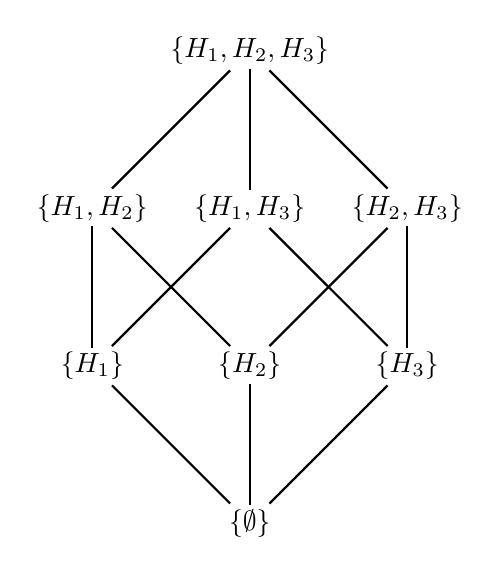
\begin{tikzpicture}
    % First, locate each of the nodes and name them
        \node (top) at (0,0) {$\{H_1, H_2, H_3\}$};
        \node (left) at (-2, -2) {$\{H_1, H_2\}$};
        \node (center) at (0, -2) {$\{H_1, H_3\}$};
        \node (right) at (2, -2) {$\{H_2, H_3\}$};
        \node (one) at (-2, -4) {$\{H_1\}$};
        \node (two) at (0, -4) {$\{H_2\}$};
        \node (three) at (2, -4) {$\{H_3\}$};
        \node (empty) at (0, -6) {$\{\emptyset \}$};

    % Now draw the lines:
        \draw [thick, shorten <=-2pt, shorten >=-2pt] (top) -- (left);
        \draw [thick, shorten <=-2pt, shorten >=-2pt] (top) -- (center);
        \draw [thick, shorten <=-2pt, shorten >=-2pt] (top) -- (right);
        \draw [thick, shorten <=-2pt, shorten >=-2pt] (left) -- (one);
        \draw [thick, shorten <=-2pt, shorten >=-2pt] (left) -- (two);
        \draw [thick, shorten <=-2pt, shorten >=-2pt] (center) -- (one);
        \draw [thick, shorten <=-2pt, shorten >=-2pt] (center) -- (three);
        \draw [thick, shorten <=-2pt, shorten >=-2pt] (right) -- (two);
        \draw [thick, shorten <=-2pt, shorten >=-2pt] (right) -- (three);
        \draw [thick, shorten <=-2pt, shorten >=-2pt] (one) -- (empty);
        \draw [thick, shorten <=-2pt, shorten >=-2pt] (two) -- (empty);
        \draw [thick, shorten <=-2pt, shorten >=-2pt] (three) -- (empty);
    \end{tikzpicture}   
    \caption{A Hasse Diagram for a world with 3 possible states.}
    \label{fig:hesse}
\end{figure}


A probability value in the interval $[0, 1]$ can be assigned to each possible state of the world such that $P(\mathbf{W}) = 1$, forming the opinion of a single agent in the population. It has been shown that human ability to reason under uncertainty seems to follow a probabilistic framework~\cite{Costello2014SurprisinglyJudgment}. Experiments have shown that the participants in the test followed Bayes rule, though corrupted by some noise. This assertion that people take a Bayesian approach has been contested, though the assertion that humans follow a probabilistic reasoning framework is supported~\cite{Douven2018CanAway}. This allows the exchange and evolution of beliefs to be modelled mathematically. 

In the field of opinion dynamics, there are two primary approaches to communication in multi-agent populations. In both, an individual agent $x$ and a subset of the population $y$ are selected at random. $x$ then queries $y$ and receives their entire set of beliefs in response. It is assumed that the population aims to confer and collectively reach a conclusion that is most beneficial to the group as a whole~\cite{Rawls1971AJustice}. The first approach describes various methods for pooling the responses together in order to update $x$'s own beliefs~\cite{Degroot1974ReachingConsensus}. Multiple different functions have been proposed for this, each producing slight variations in the way in which the population converges to a single shared belief~\cite{Lee2018CombiningConsensus}. This pooling aims to make use of the ``wisdom of the crowd'' effect~\cite{Golub2010NaiveCrowds}. This refers to the belief that the more people involved in making a judgement, the more information is available, and so the more accurate the decision will be. However, there are those that argue that the opposite must also be true: the more people present, the more misinformation is available in the decision-making process, thus drowning out the voices of those who may be most accurate~\cite{Dalkey1963AnExperts}. There is experimental evidence in support of the ``wisdom of the crowd'' and decision-making techniques based on it, such as the Delphi Method. This is a technique employed in order to obtain the best verdict from a panel of experts~\cite{Dalkey1963AnExperts}. The method begins with the panellists completing a questionnaire in isolation without communicating with one another. These are then summarised and shown to each member of the group, who are invited to update their responses. This process is repeated until a predetermined condition is met, and shows that this combination of expert opinions often converges to a single clear idea. 

The second approach to the amalgamation of opinions is for $x$ to simplify the combination process, taking an average of each of the other agent's beliefs weighted by a parameter representing the population's view of their reliability~\cite{Hegselmann2002OpinionSimulation}. This reliability parameter can lend disproportionate influence to a small number of agents, making them dominant factors in the decision-making process. The reverse is also true, with some agents' opinions being disregarded as they are deemed unreliable. The model can be extended to include an element of $x$'s past beliefs, so that they are not lost when updated, for example, in the Friedkin Johnsen (FJ) model~\cite{Friedkin1999SocialChange}. The FJ model takes a linear combination of $x$'s previous beliefs and the weighted average of the population's beliefs, forming $x$'s updated beliefs. This method has also been trialled on humans~\cite{Friedkin2011APower}. Groups of four students were placed in separate rooms and asked to reach a decision as a group within 20 minutes. The only means of communication was a phone in each room, that could not connect to more than one person at a time. These experiments demonstrated that, generally, a single member of the group emerged as the most influential in reaching a collective decision. 

These models are advantageous because the rationale behind the decision made by the agents is interpretable by humans. However, the models can still be improved, as each agent in $y$ broadcasts more information that may be relevant. The complexity in these models is in the behaviour of $x$ upon receipt of new information from $y$. 

\section{Aims and Motivation}

This project aims to explore the effects of including aspects of persuasion into communication in multi-agent systems. It is important that the population be able to converge to a unanimous agreement in a single shared belief. Without such a consensus, the agents are unable to achieve their full potential, and may fail to reach their intended goal. A secondary aim of this work is to provide a structure to the evolution of beliefs in artificial populations. With such a structure, it is possible to more easily explain the rationale behind an agent's communication, and interpret the opinion dynamics of the system. 


\section{Plan of the Report}

In this report, we adopt a simple probabilistic model of beliefs and a speaker-listener model for communication. One agent is selected at random to broadcast a persuasive argument and another is chosen as the listener that must react to the argument at each iteration. \Cref{sect:method} outlines the experimental set up for the models that are described in \cref{sect:speaker_models} and ~\cref{sect:listener_models}. \Cref{sect:analysis} discusses the results found before suggesting a number of extensions to the experimental setup that aim to more closely mimic human behaviours, incorporating aspects of persuasion. This work is concluded with a discussion of the main results and a number of avenues for further work. 









